% THIS IS THE LATEX CODE WHICH GENERATED THE POSTER: 

% Ref: https://www.overleaf.com/latex/templates/emory-poster-template/skpfmpxjnqdh

\documentclass[25pt, a0paper, portrait, margin=10mm, innermargin=15mm, blockverticalspace=10mm, subcolspace=7mm, dvipsnames]{tikzposter} % you need to leave in dvipsnames or else it undoes the orange edge colour??

\usepackage{tikz}
\usetikzlibrary{shapes,arrows,positioning,fit,backgrounds,calc}
\usepackage[T1]{fontenc}
\usepackage{helvet}
%\usepackage[utf8]{inputenc}
\usepackage{amsmath}
\usepackage{amsfonts}
\usepackage{amsthm}
\usepackage{amssymb}
\usepackage{siunitx}
\usepackage{mathrsfs}
\usepackage{url}
\usepackage{graphicx}
\usepackage{adjustbox}
\usepackage{enumitem}
\usepackage[font=small,skip=0pt]{caption}
%  nature style bins DOIs, more compact
\usepackage[backend=biber, style=nature, citestyle=ieee, url=false, isbn=false]{biblatex}
\usepackage{xpatch}
\usepackage{xcolor}
\usepackage{multicol}
\usepackage{lipsum}
\usepackage{setspace}
\usepackage{tcolorbox}
\usepackage{wrapfig}
\addbibresource{references.bib}
\setlength{\columnsep}{2cm}
\setlength{\columnseprule}{1mm}
\pagecolor{Dandelion}

% Ref: https://latex-cookbook.net/poster/
\renewcommand*{\familydefault}{\sfdefault}% Let's have a sans serif font

% set theme parameters
\tikzposterlatexaffectionproofoff
\usepackage{anyfontsize}
\usetheme{Default}
\usebackgroundstyle{Default}
\definecolor{epccnavy}{HTML}{1D2A3D}
\definecolor{universityred}{HTML}{D50032}
\colorlet{backgroundcolor}{white} % <<< this makes bg white
\colorlet{framecolor}{epccnavy}%Dandelion}
\colorlet{titlefgcolor}{epccnavy}
\colorlet{blocktitlebgcolor}{epccnavy}
\colorlet{blocktitlefgcolor}{white}
\colorlet{blockframecolor}{epccnavy}


% Ref: https://tex.stackexchange.com/questions/309713/modify-font-style-in-title-of-tikzposter
\settitle{ \raggedright
\hspace{-6em}  
% make title text block go left!
\vbox{
    \begin{spacing}{1.2}
    %\@titlegraphic \\[\TP@titlegraphictotitledistance] \centering
    \color{titlefgcolor} {\sffamily \bfseries \huge  \textsc{\@title} \par}
    \vspace*{0.75em}
    \color{universityred} {\sffamily \bfseries \huge \subtitle}   
    %\vspace*{0.2em}
    \begin{flushleft}
    {\color{titlefgcolor} {\sffamily \huge \@author}
    \hspace{0.2em}
    {\sffamily \LARGE \@institute \par}}
    \end{flushleft}   
    \end{spacing}
}
}
\makeatother

% Ref: https://tex.stackexchange.com/questions/180234/how-can-i-make-my-title-wrap-in-a-tikzposter
\makeatletter
\def\title#1{\gdef\@title{\scalebox{\TP@titletextscale}{%
			\begin{minipage}[t]{\linewidth}
				%\centering
				#1
			\par
				\vspace{0.5em}
			\end{minipage}%
}}}
\makeatother

% Ref: https://tex.stackexchange.com/questions/263563/add-logos-beyond-the-title-tikzposter
\title{\parbox{\linewidth}{\fontseries{bx}\selectfont {\fontsize{82}{84}\selectfont {Who Do You Think You Are?} }}}
\newcommand{\subtitle}{Identifying Research Software Engineering Personas From Developer / Repository Interaction Data}
\author{\textbf{Felicity `Flic' Anderson\textsuperscript{$\dagger$}\textsuperscript{$\star$}, Dr. Julien Sindt\textsuperscript{$\dagger$} \& Prof. Neil Chue Hong\textsuperscript{$\dagger$}}}
\institute{\textsuperscript{$\dagger$}EPCC, University of Edinburgh \hspace{5em}
\textsuperscript{$\star$}\url{Felicity.Anderson@ed.ac.uk}}


\makeatletter
\newcommand\insertlogoi[2][]{\def\@insertlogoi{\includegraphics[#1]{#2}}}

\newcommand\insertlogoii[2][]{\def\@insertlogoii{\includegraphics[#1]{#2}}}

\newlength\LogoSep
\setlength\LogoSep{0pt}

\insertlogoi[width=12cm]{posterlogos.pdf}
% \insertlogoii[width=10cm]{epcclogo.png}
%\insertlogoii[width=15cm]{EpccANDEmailQRsidebyside.png}

\renewcommand\maketitle[1][width=600mm, linewidth=6pt]{  % #1 keys
	\normalsize
	\setkeys{title}{#1}
	% Title dummy to get title height
	\node[transparent,inner sep=\TP@titleinnersep, line width=\TP@titlelinewidth, anchor=north, minimum width=\TP@visibletextwidth-2\TP@titleinnersep]
	(TP@title) at ($(0, 0.5\textheight-\TP@titletotopverticalspace)$) {\parbox{\TP@titlewidth-2\TP@titleinnersep}{\TP@maketitle}};
	\draw let \p1 = ($(TP@title.north)-(TP@title.south)$) in node {
		\setlength{\TP@titleheight}{\y1}
		\setlength{\titleheight}{\y1}
		\global\TP@titleheight=\TP@titleheight
		\global\titleheight=\titleheight
	};
	
	% Compute title position
	\setlength{\titleposleft}{-0.6\titlewidth}
	\setlength{\titleposright}{\titleposleft+\titlewidth}
	\setlength{\titlepostop}{0.5\textheight-\TP@titletotopverticalspace}
	\setlength{\titleposbottom}{\titlepostop-\titleheight}
	
	% Title style (background)
	\TP@titlestyle
	
	% Title node
	\node[inner sep=\TP@titleinnersep, line width=\TP@titlelinewidth, anchor=north, minimum width=\TP@visibletextwidth-2\TP@titleinnersep]
	at (0,0.5\textheight-\TP@titletotopverticalspace)
	(title)
	{\parbox{\TP@titlewidth-2\TP@titleinnersep}{\TP@maketitle}};

	\node[inner sep=0pt,anchor=east,yshift=0cm] 
	at ([xshift=\LogoSep]title.east)
	{\@insertlogoi};
	
	% Settings for blocks
	\normalsize
	\setlength{\TP@blocktop}{\titleposbottom-\TP@titletoblockverticalspace}
}
\makeatother

\onehalfspacing
% begin document
\begin{document}
%\useblockstyle{Basic}
\maketitle
\begin{columns}
\column{.5}

\block[linewidth=5pt]{0: RSE Personas from GitHub Data}{
    {\fontsize{32}{34}\selectfont
    We mined 45 GitHub repositories to attempt to identify \textbf{data-driven RSE Personas} for 791 contributors. \par
    \vspace{0.5em}
    We hypothesised 4 main RSE Personas (Fig.\ref{fig:hypothesised-personas});
    we can confirm \textbf{`Active Leaders'} and \textbf{`Occasional Contributors'}, others are less clear...\par
    }
}

\block[linewidth=5pt]{1: How to Create Data-Driven RSE Personas}{ 
    \begin{multicols}{2}
    {\fontsize{28}{28}\selectfont    
    \begin{tikzfigure}[\normalsize Data gathering workflow.\par]
    \setlength{\belowcaptionskip}{-16pt}
        \label{fig:workflow}
        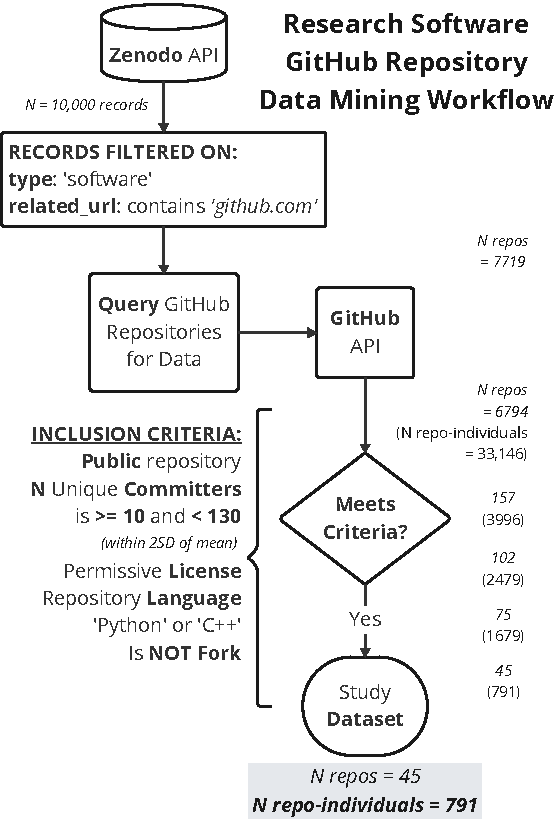
\includegraphics[width=1\linewidth]{Figures/dataminingworkflow.pdf}
    \end{tikzfigure}
    Zenodo was used to source for GitHub repositories with a DOI.\par
    \vspace{0.2em}
    \begin{tikzfigure}[Hypothesised RSE Personas.]
    \setlength{\belowcaptionskip}{-8pt}
        \label{fig:hypothesised-personas}
        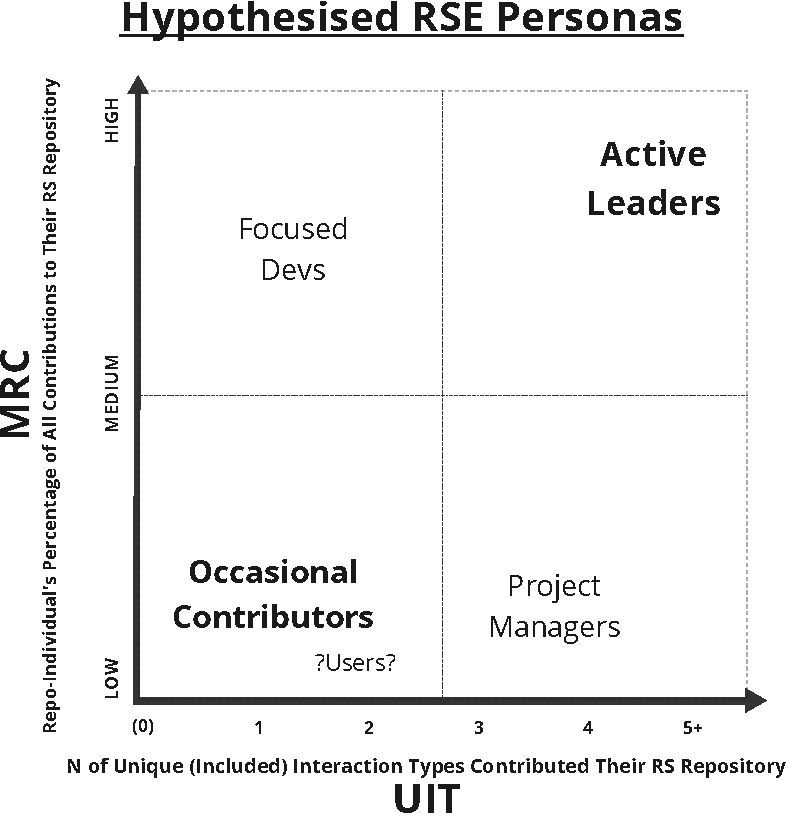
\includegraphics[width=1\linewidth]{Figures/hypotheses-quadrant.pdf}
    \end{tikzfigure}
    \vspace{0.2em}
    Repositories in the dataset contained a \textbf{mean of 18 repo-individuals} (min=10, max=50).
    Repository interactions were analysed across variables (see Fig.\ref{fig:variables})
    \columnbreak
    % \columnbreak 
    \begin{tikzfigure}[]
    \setlength{\belowcaptionskip}{-8pt}
            \label{fig:interactive}
            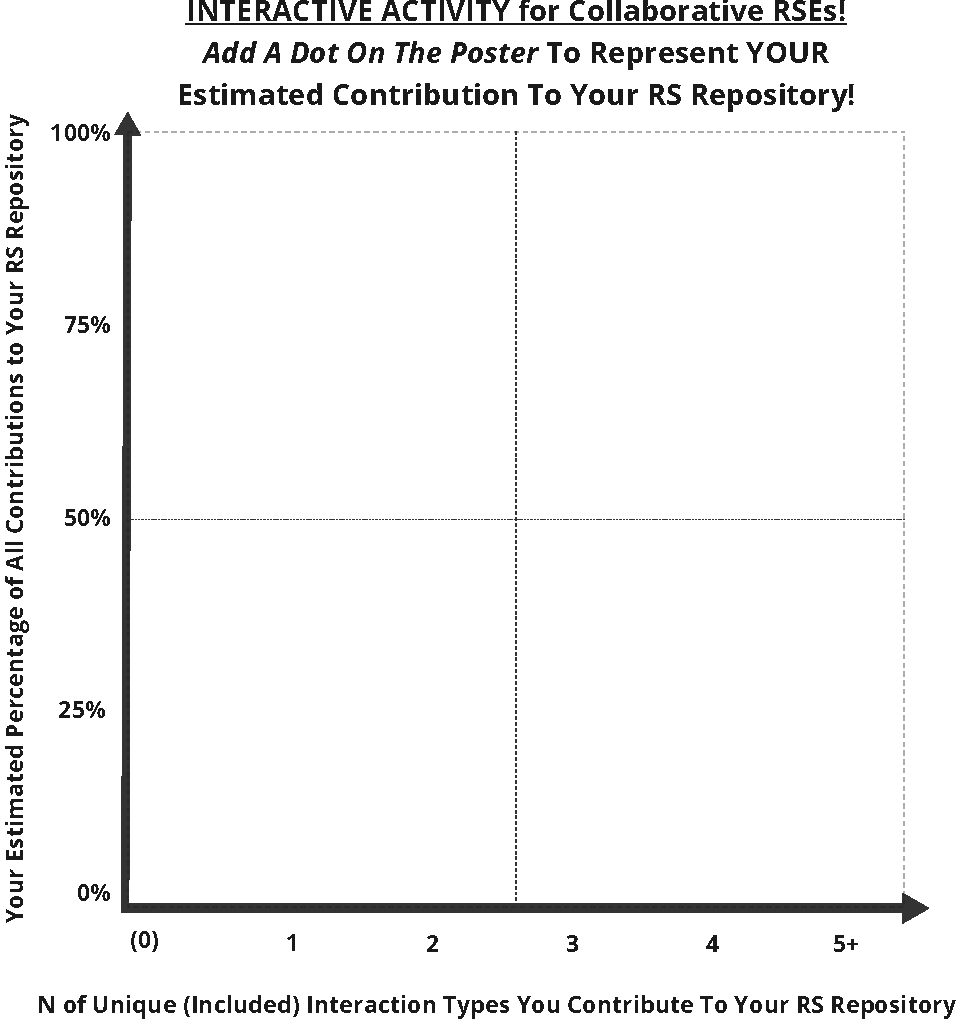
\includegraphics[width=1\linewidth]{Figures/interactive_activity.pdf}
    \end{tikzfigure}
    approximating \textit{`depth' (MRC)} and \textit{`breadth' (UIT)} of contributions.\par
    \vspace{0.3em}
    \textbf{Hierarchical Clustering} identified \textbf{3 clusters} (Fig.\ref{fig:dendrogram}: Calinski–Harabasz index 757.60, N=3 clusters) from similarities across interaction data. \par
    \begin{tikzfigure}[Dendrogram for Hierarchical Clustering using Ward method and Euclidean distance.]
         \setlength{\belowcaptionskip}{-8pt}
         \label{fig:dendrogram} 
        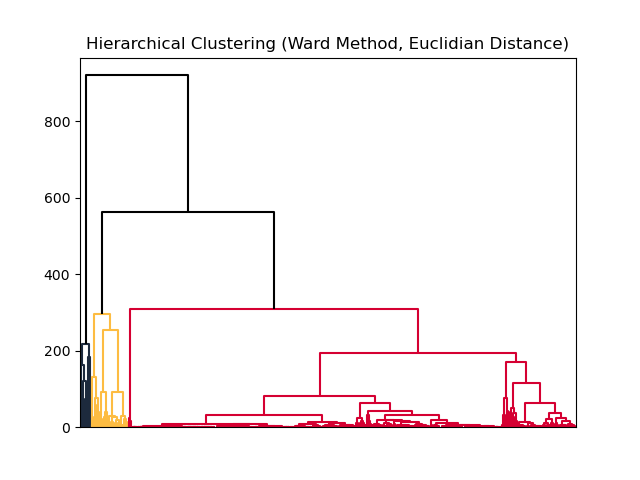
\includegraphics[width=0.98\linewidth]{Figures/dendrogram_ward_euclidian_x45repos_x791project_individuals_2025-02-18.png}
    \end{tikzfigure}   
    714 repo-individuals fall into one cluster category, with the remaining 77 across two remaining categories. 
    \textbf{Cluster 0: 90.27\%}, (red); \textbf{Cluster 2: 7.46\%}, (gold);  \textbf{Cluster 1: 2.28\%}, (navy). \par
    \vspace{0.2em}
    Cluster diversity was moderate: 84.4\% (38) of the 45 repositories contain RSEs from 2 clusters. 6 (13.3\%) had all clusters, 1 repo\-sitory contained only a single cluster. \par 
    }
    \end{multicols}
    \vspace{0.35em}
    \begin{tikzfigure}[Key variable definitions and relationship to hypotheses.]
        \label{fig:variables}
        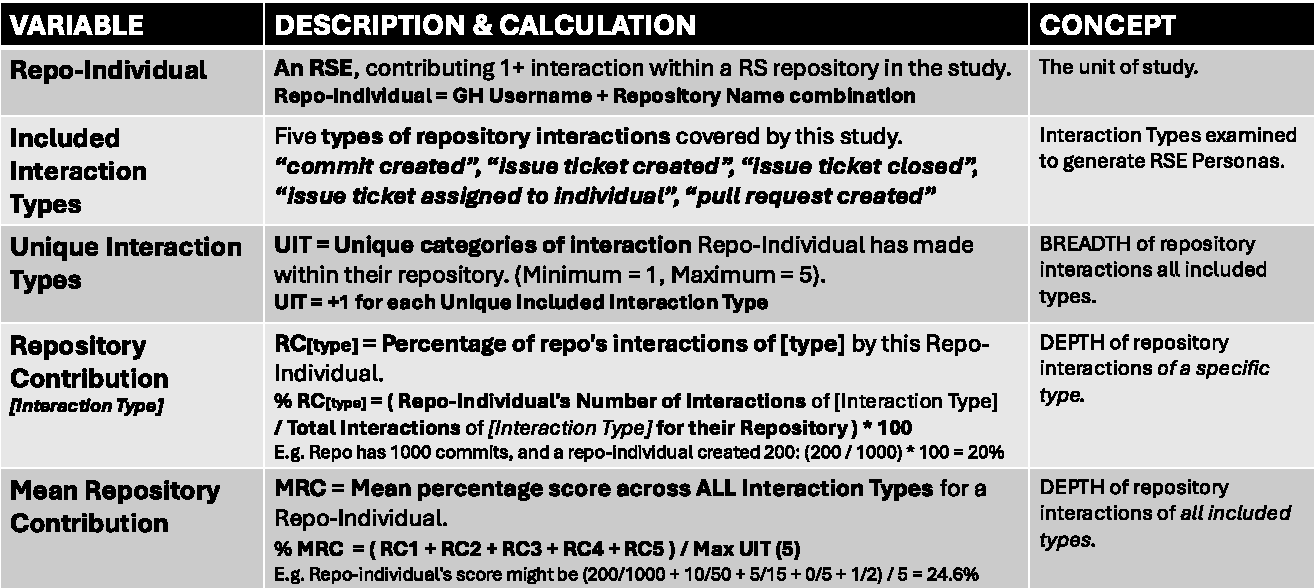
\includegraphics[width=1\linewidth]{Figures/variables-short.pdf}
    \end{tikzfigure}
}

\column{.5}
\block[linewidth=5pt]{2: Identifying (with) RSE Personas}{
    {\fontsize{29}{29}\selectfont 
    \begin{multicols}{2}
    \begin{tikzfigure}[RC values for Commit Creation and Pull (PR) Request Creation, across UIT.]
            \label{fig:commit-pr-rcs}
    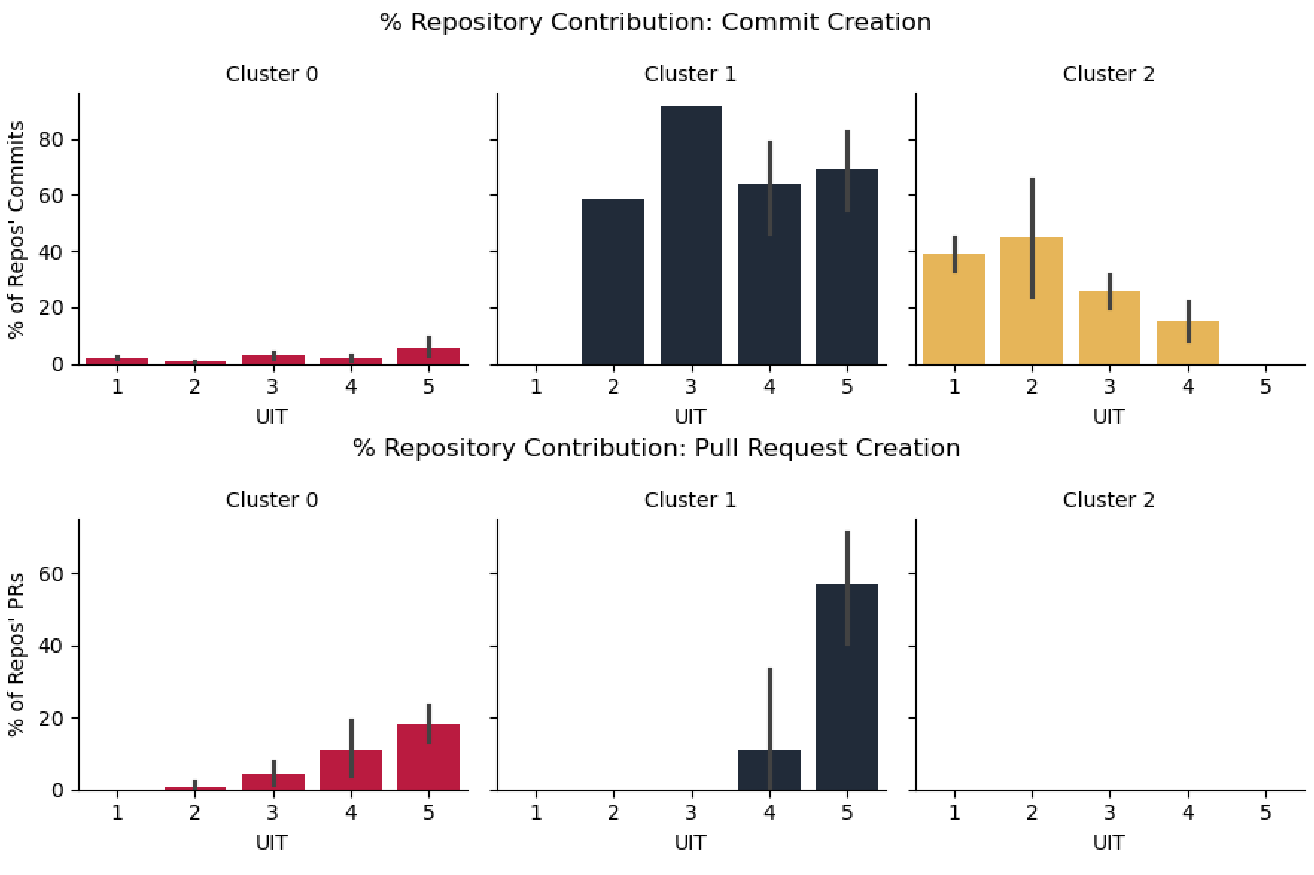
\includegraphics[width=1\linewidth]{Figures/rc-commits-prs.pdf}
    \end{tikzfigure} 
    \vspace{0.2em}
    Fig.\ref{fig:commit-pr-rcs} shows contrasting patterns of behaviours between clusters for committing and PRs, supported by ANOVA results (p < 0.001). \par
     \begin{tikzfigure}[Distribution of Repo-Individuals across UIT.]
    %\setlength{\belowcaptionskip}{-8pt}
    \label{fig:uit}
        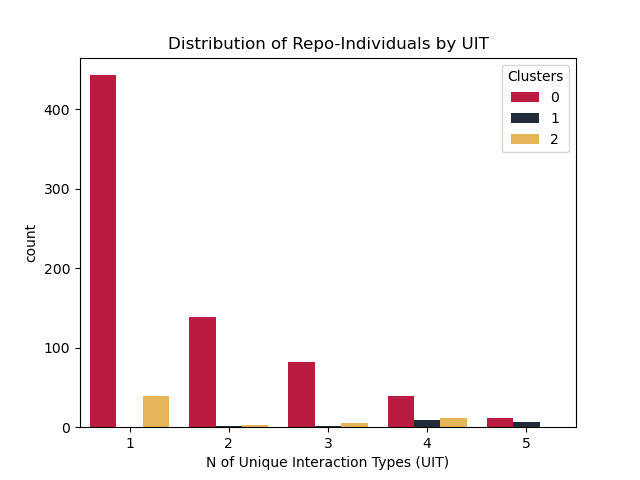
\includegraphics[width=1\linewidth]{Figures/UIT_distribution_2025-02-20.png}
    \end{tikzfigure} 
    \vspace{0.2em}
    Fig.\ref{fig:uit} indicates the majority of repo-individuals only contribute to 1 UIT. 
    These are the 482 (60.9\%) RSEs from 41 repositories who only create commits. 
    Conversely, only 18 (2.3\%) repo-individuals displayed interactions from all valid interaction types. \par
    
    \begin{tikzfigure}[MRC highly significant (p < 0.001) by Cluster.]
    %\setlength{\belowcaptionskip}{-8pt}
    \label{fig:mrc}
        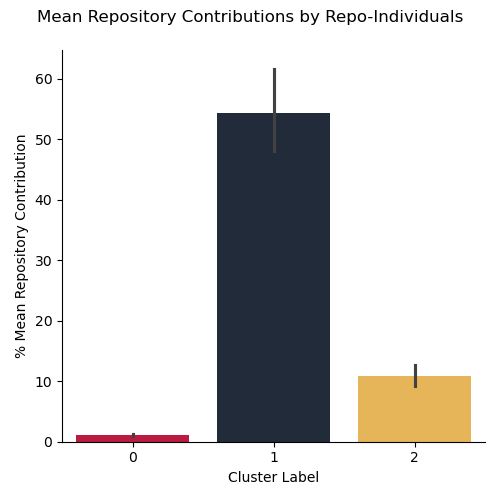
\includegraphics[height=1\linewidth]{Figures/mrc_cluster_2025-02-20.png}
    \end{tikzfigure}    
    Differences in MRC between clusters are highly significant (p < 0.001) across all relationships (Fig.\ref{fig:mrc}). \par
    %: p=1.14 x10\textsuperscript{-288}.
    \begin{tikzfigure}[Variation in \% MRC across UIT.]
    %\setlength{\belowcaptionskip}{-8pt}
    \label{fig:uit-mrc}
        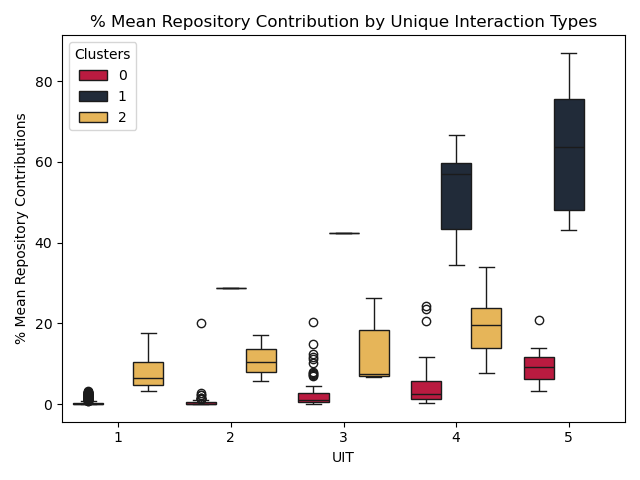
\includegraphics[width=1\linewidth]{Figures/uit_mrc_cluster_2025-02-20.png}
    \end{tikzfigure}   
    ANOVA and Tukeys HSD tests identify MRC varying significantly across UIT categories (p < 0.001), while low:high pairings of UIT are highly significant. \par
    \end{multicols}

    }
}
\block[linewidth=5pt]{3: Evaluating RSE Personas Approach}{
    {\fontsize{28}{28}\selectfont 
    \begin{tcolorbox}[colframe=white,colback=epccnavy!25, linewidth=0.8*linewidth]{
    \textbf{Active Leaders map to Cluster 1} as a RSE Persona type with \textbf{high UIT and high MRC} values (Fig.\ref{fig:uit-mrc}). 
    Despite rarity (2\% of repo-individuals), they generate >50\% their repositories' interactions. \par

    \vspace{0.2em}

    \textbf{Cluster 0 maps well to hypothesised `Occasional Contributors'}, showing low `MRC' values and skewing strongly to very low `UIT'. 
    Could be examined for possible sub-clusters.\par

    \vspace{0.4em}

    \textbf{`Focused Developers' RSE Persona was disproved} by no clusters with high MRC and low UIT, so is rejected as hypothesised.\par

    \vspace{0.3em}
    
    The \textbf{`Project Managers'} RSE Persona is rejected as unclear - Cluster 2 does occupy the low MRC space, but may show possible bimodality in relation to UIT. \par
    }
    \end{tcolorbox}

    \textbf{Variables `MRC' and `RC pull-request-created' are significant} and explain high variance in Principal Component Analysis (PCA), acting as a robust basis for RSE Personas. 
    \textbf{UIT does not explain cluster variance well}.
    This could be due to the differing `combinations' of interactions confusing the picture.\par
    
    \vspace{0.4em}
    \textbf{Ask Me About Limitations...} 
    Skews towards 'best practices'; not all interactions are equal; project comparison difficulties; capturing changes over time; real-world validity-checking...\par
    }
}
    
\block[linewidth=5pt]{4: Using RSE Personas}{
    %     %\vspace{1em}
    {\fontsize{28}{28}\selectfont
    \textbf{Next Steps...} 
    Include more UITs (code review, discussions, merges); compare other languages - data vs HPC?; explore time and commit category data more deeply... \par
    \vspace{0.4em}
    \textbf{Future Work...}
    \textit{RSE Persona dynamics} - co-occurrences or limiting factors?; \textit{RSE Persona Fluidity} - do personas change over time/repos?); \textit{create Taxonomy of RSE Personas} with descriptive characteristics to aid usage.\par
    }
}
\end{columns}
\block[linewidth=5pt]{}{
\centering
\begin{multicols}{2}
    {\fontsize{28}{28}\selectfont
    \textbf{github.com/FlicAnderson/RSE-Personas-Who
    } \par
    % \textbf{Contact: 
    % \hspace{0.5em}
    % Felicity.Anderson@ed.ac.uk} \par 
    \textbf{Acknowledgements:} 
    \hspace{0.5em}
    Work funded by EPSRC DTA Scholarship. \par
    }
    \end{multicols}
}
\end{document}
